\section{Styrenhet}

Styrenhetens huvudsakliga uppgift är att ta emot data från
kommunikationsenheten och omvandla det till PWM signaler som styr motorerna.
Styrningen av motorerna sker antingen autonomt med reglering eller 
manuellt genom styrkommandon.

\subsection{Hårdvara}

Styrenheten består av en AVRAtmega16 som sänder styrsignalerna till motorerna, 
En brytknapp som väljer mellan autonomt och manuellt läge, en startknapp och en 
resetknapp.  

\begin{figure}[H]
  \centering
 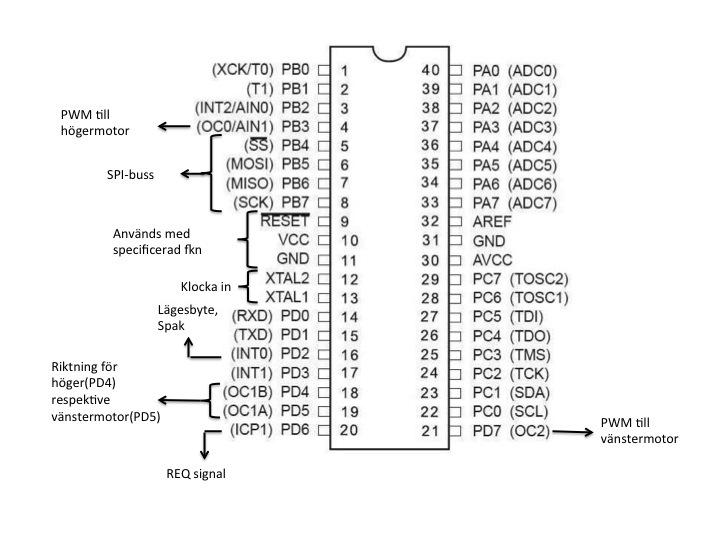
\includegraphics[angle=0,scale=0.5]{bilder/PIN_styr.jpg}
  \caption{Styrenhetens pin-anslutningar}
  \label{fig:PINstyr}
\end{figure}


\subsection{Mjukvara}

\subsubsection{Autonomt läge}

\subsection{Reglering}
Två olika regleralgoritmer används i roboten, en när roboten följer linjer och
en när roboten kör i labyrinter.
\subsubsection{Linjereglering}
Utöver att uppfatta var på linjen roboten för närvarande befinner sig är 
linjeregleringen är anpassad för att uppfatta i vilken riktning roboten för 
närvarande färdas. Datan som styrenheten tar emot när roboten befinner sig i 
linjeläge innehåller en kod som visar vilken sensor som är närmast mitten på 
tejpen. Är 2 sensorer för närvarande på tejpen väljs den längst åt höger. 
Koden kan vara något av 11 diskreta värden som sträcker sig från -127 till 127.

Då detta värde ändras så bestäms i vilken riktning relativt tejpen som 
roboten för närvarande rör sig. Detta avgör sedan hur roboten ska bete sig.

Kommer roboten in högerifrån, och tejpen ligger över de högra sensorerna 
utförs en en vänstersväng som blir kraftigare ju närmare de vänstra 
sensorerna roboten kommer. Utförandet är detsamma, fast motriktat, om roboten 
kommer in vänsterifrån, och tejpen ligger över de vänstra sensorerna.

Kommer roboten in vänsterifrån, och tejpen ligger över de vänstra sensorerna 
så utförs en kraftig sväng som avtar när tejpen närmar sig de högra sensorerna
.Utförandet är detsamma, fast motriktat, om roboten kommer in högerifrån, och 
tejpen ligger över de högra sensorerna.


Linjeregulatorn har utöver detta flera olika egenskaper för att förbättra 
regleringen:
\begin{itemize}
\item Visar linjesensorerna att samma sensor varit mitt över tejpen i mer än 8st avläsningar, så utgår regulatorn ifrån att tejpen för tillfället är rak och roboten beordras att röra sig rakt framåt. Under de första 8 avläsningarna som samma sensor varit i mitten av tejpen så utgår regulatorn att roboten har samma riktning relativt tejpen som tidigare.
\item Visar linjesensorerna att att mitten av tejpen rört sig än 2 sensorer eller mer under de senaste 20 avläsningar, så dubblas regulatorns "effekt".
\item Om roboten hamnat utanför tejpen, det vill säga att den av någon anledning kört av, så svänger regulatorn kraftigt åt den riktning där tejpen senast uppfattats
\end{itemize}



\subsubsection{Labyrintreglering}
Labyrintregleringen består av 3 olika delar med olika vikter,
en del som ser till att roboten går rakt (P-del), en del som ser till att
roboten håller sig i mitten av labyrinten (M-del) och en del som motverkar
svängningar (D-del).


P-delen använder sig av sidosensorerna för att hålla roboten parallell med
labyrintväggen. En vägg följs i taget, och kommer roboten för nära en vägg så
följs istället den andra väggen. Detta är den huvudsakliga regleringen och har
hög vikt.


M-delen använder sig av frontsensorerna för att hålla sig i mitten av
labyrinten, den försöker att hålla skillnaden mellan höger- och vänstersensorn
till 0. Om det bara finns en vägg att reglera på avaktiveras denna del. Då det
inte är helt avgörande om roboten är i mitten eller lite åt sidan i labyrinten
har denna del låg vikt.


D-delen ser till att roboten rör sig lugnt och inte börjar att oscillera i
labyrinten. Detta gör den genom att kika på skillnaden på sidosensorerna och är
den skillnaden stor så motverkar den P-delen. Eftersom D-delen reglerar på
relativt små skillnader har den hög vikt.

\label{reglering}
